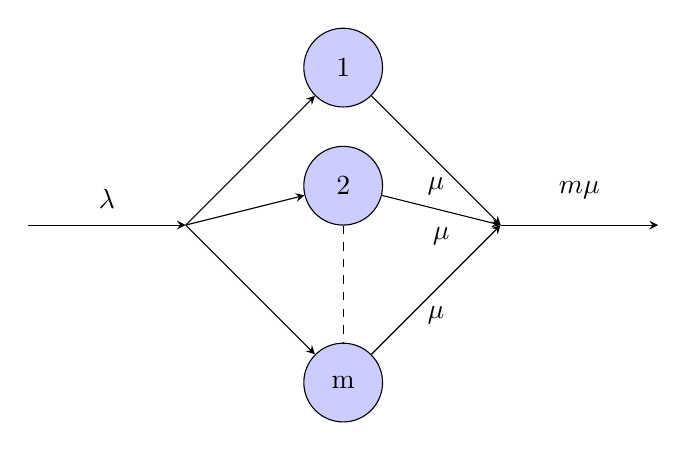
\begin{tikzpicture}[>=stealth, node distance=1.5cm, every node/.style={circle}]
    % Nodes
    \node (1) [{draw, fill=blue!20, minimum size=10mm, inner sep=0pt}]{1};
    \node (2) [{below of=1, draw, fill=blue!20, minimum size=10mm, inner sep=0pt}] {2};
    \node (m) [{below of=2, yshift=-1cm, draw, fill=blue!20, minimum size=10mm, inner sep=0pt}] {m};

    % Arrows for transitions
    \draw[->] (-2, -2) -- (1); 
    \draw[->] (-2, -2) -- (2); 
    \draw[->] (-2, -2) -- (m); 
    \draw[->] (1) -- (2, -2) node[midway, below] {$\mu$};
    \draw[->] (2) -- (2, -2) node[midway, below] {$\mu$};
    \draw[->] (m) -- (2, -2) node[midway, below] {$\mu$}; 

    % Connecting lines between nodes
    \draw[dashed] (2) -- (m);

    % Lambda arrow entering the chain
    \draw[->] (-4, -2) -- (-2, -2) node[midway, above] {$\lambda$};
    \draw[->] (2, -2) -- (4, -2) node[midway, above] {$m \mu$};
    
\end{tikzpicture}